\section{Presentation Logic Layer}

%What pages will be present in your project? briefly indicate how your web site will be organized

Here are listed the main pages that will be available on our web application:

\begin{itemize}
    \item Login Page: here the user can log in filling the form with his username and password;
    \item Home Page: the home page of the application: the home page will be reached immediately after the login part. Here some of the insight plots will be displayed. on the left side of the page a nav menu will be shown, with the dropdown menu that will allow to choose the current company used, and all other following sections will be displayed as links;
    \item User Page: here the user can access to his reserved area, in which will able to modify user settings, notification settings, company settings and bank account settings through forms;
    \item Product Creation Page: here the user will have a form to insert a new product in the database;
    \item Product Update Page: here the user will have firstly the possibility to choose one of his products through a radio button: once one is chosen, he will be redirected to a pre-filled form of the product, in which he will be able to modify it;
    \item Product Delete Page: here the user will have the possibility to delete a product, through a radio button;
    \item Product List Page: here a list of all products will be listed: a button will allow the user to download in pdf format a list of all the products;
    \item Customer Creation Page: here the user will have a form to insert a new customer in the database;
    \item Customer Update Page: here the user will have firstly the possibility to choose one of his customers through a radio button: once one is chosen, he will be redirected to a pre-filled form of the customer, in which he will be able to modify it;
    \item Customer Delete Page: here the user will have the possibility to delete a customer, through a radio button;
    \item Customer List Page: here a list of all customers will be listed: a button will allow the user to download in pdf format a list of all the customers;
    \item Invoice Creation Page: here a new invoice entity will be created, setting up some general data through a form, as for example to which customer the invoice will be related;
    \item Invoice Update Page: here the user can edit the data entered in the creation part;
    \item Invoice List Page: here the user can look to the list of his invoices, in which he will see all the open invoices, in which he will able to add invoice rows, closed invoices that are waiting to be billed (invoice warning PDF will be available for download), and billed invoices (actual invoice in both PDF and XML will be available for download). Filters to the list will be available.
    \item Invoice Row List Page: by clicking on an invoice a list of all invoice rows of a specific invoice will be available;
    \item Invoice Row Insertion Page: by clicking on a specific button on open invoices, a form to insert a new row on the invoice will be available, in which also the product sold will be available;
    \item Detailed Insights Page: a page where the user can see all the insights available.
\end{itemize}
\newpage
\subsection{Login page - Reset password page - New password page}

Description


%For the main pages put a mockup and describe it in detail.
\begin{figure}[h!]
    \centering
    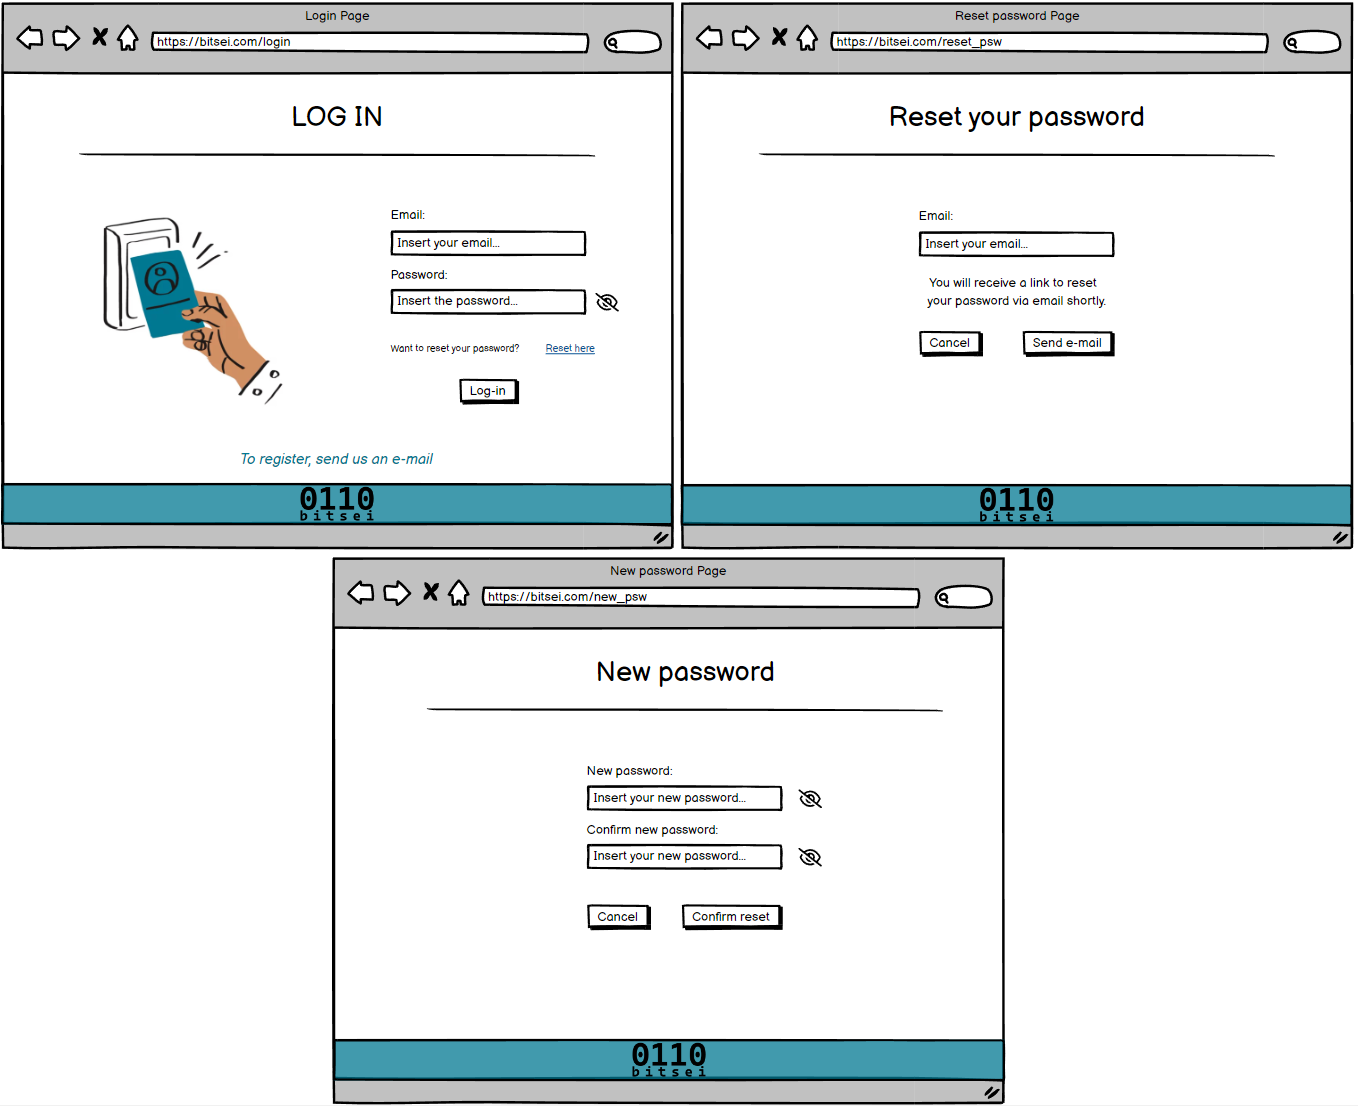
\includegraphics[height=390pt, keepaspectratio]{resources/mockup/Login.png}
\end{figure}
\newpage
\subsection{Home page}

Description


%For the main pages put a mockup and describe it in detail.
\begin{figure}[h!]
    \centering
    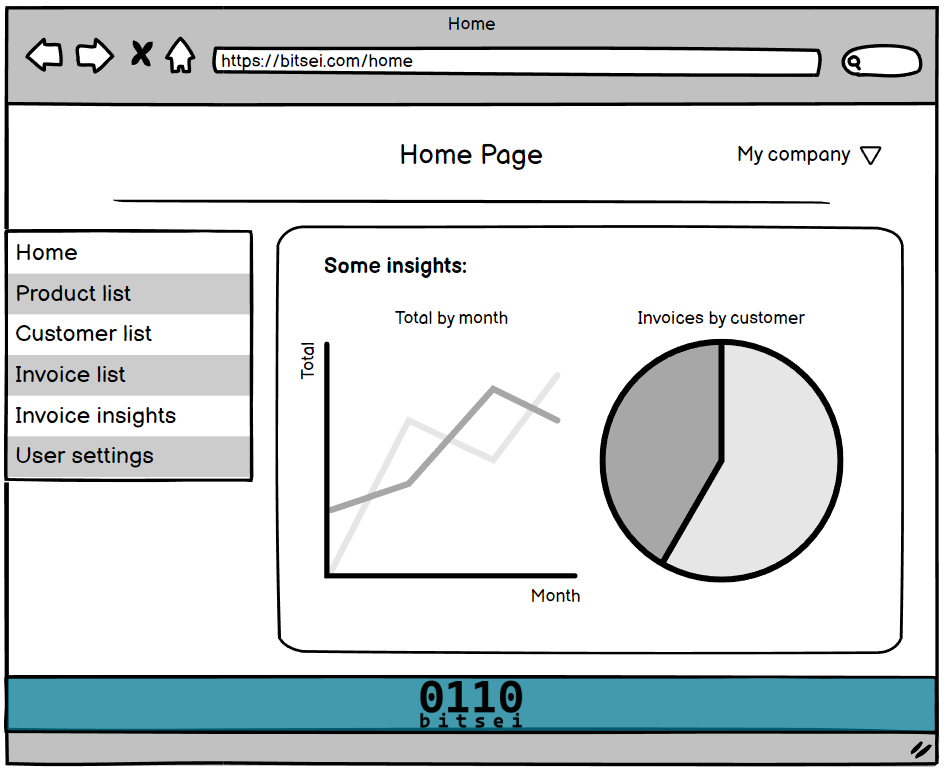
\includegraphics[height=380pt, keepaspectratio]{resources/mockup/Home.png}
\end{figure}
\newpage
\subsection{Invoice list page}

Description

%For the main pages put a mockup and describe it in detail.
\begin{figure}[h!]
    \centering
    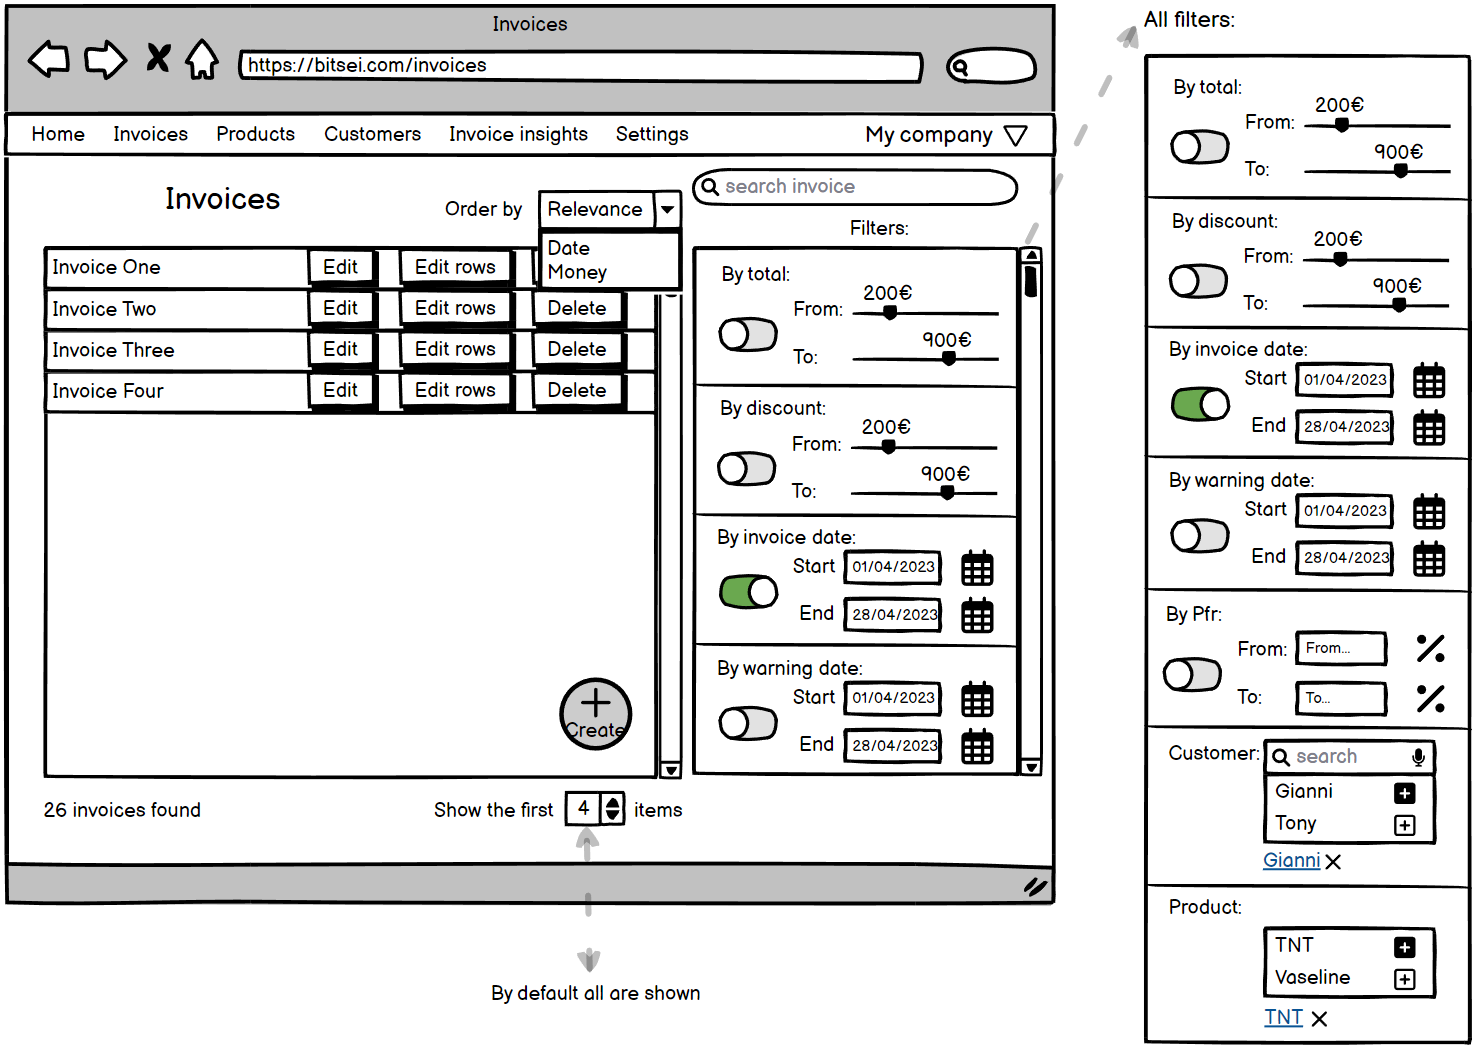
\includegraphics[height=340pt, keepaspectratio]{resources/mockup/Invoice_list.png}
\end{figure}
\newpage
\subsection{Create invoice page - Edit invoice page - Invoice rows page}

Description

%For the main pages put a mockup and describe it in detail.
\begin{figure}[h!]
    \centering
    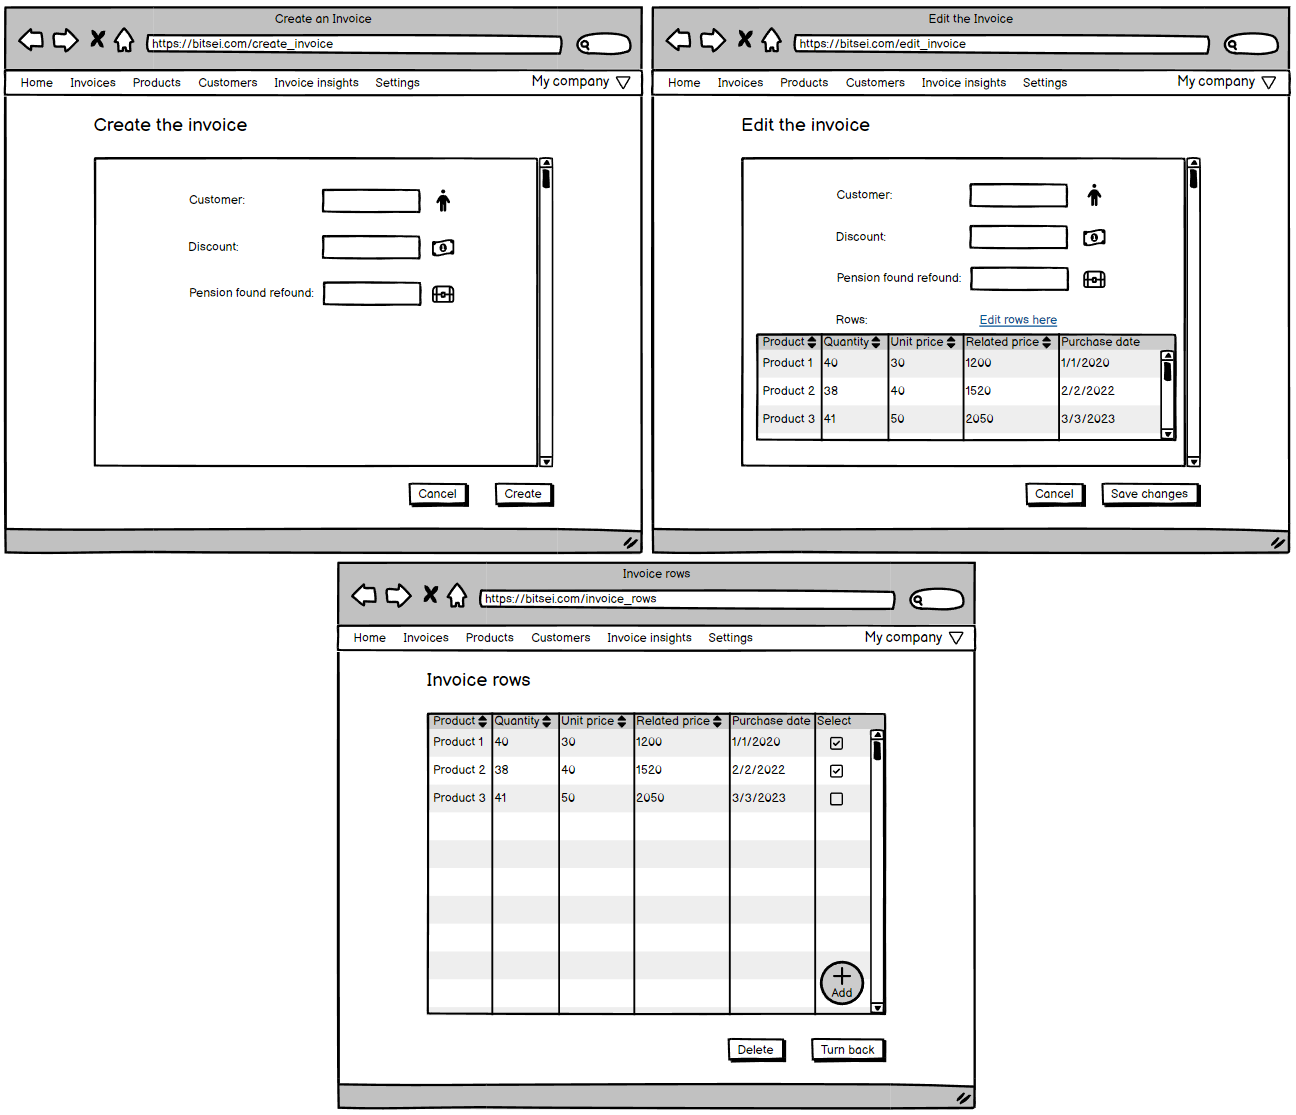
\includegraphics[height=400pt, keepaspectratio]{resources/mockup/Invoice.png}
\end{figure}
\newpage
\subsection{Invoice details page}

Description

%For the main pages put a mockup and describe it in detail.
\begin{figure}[h!]
    \centering
    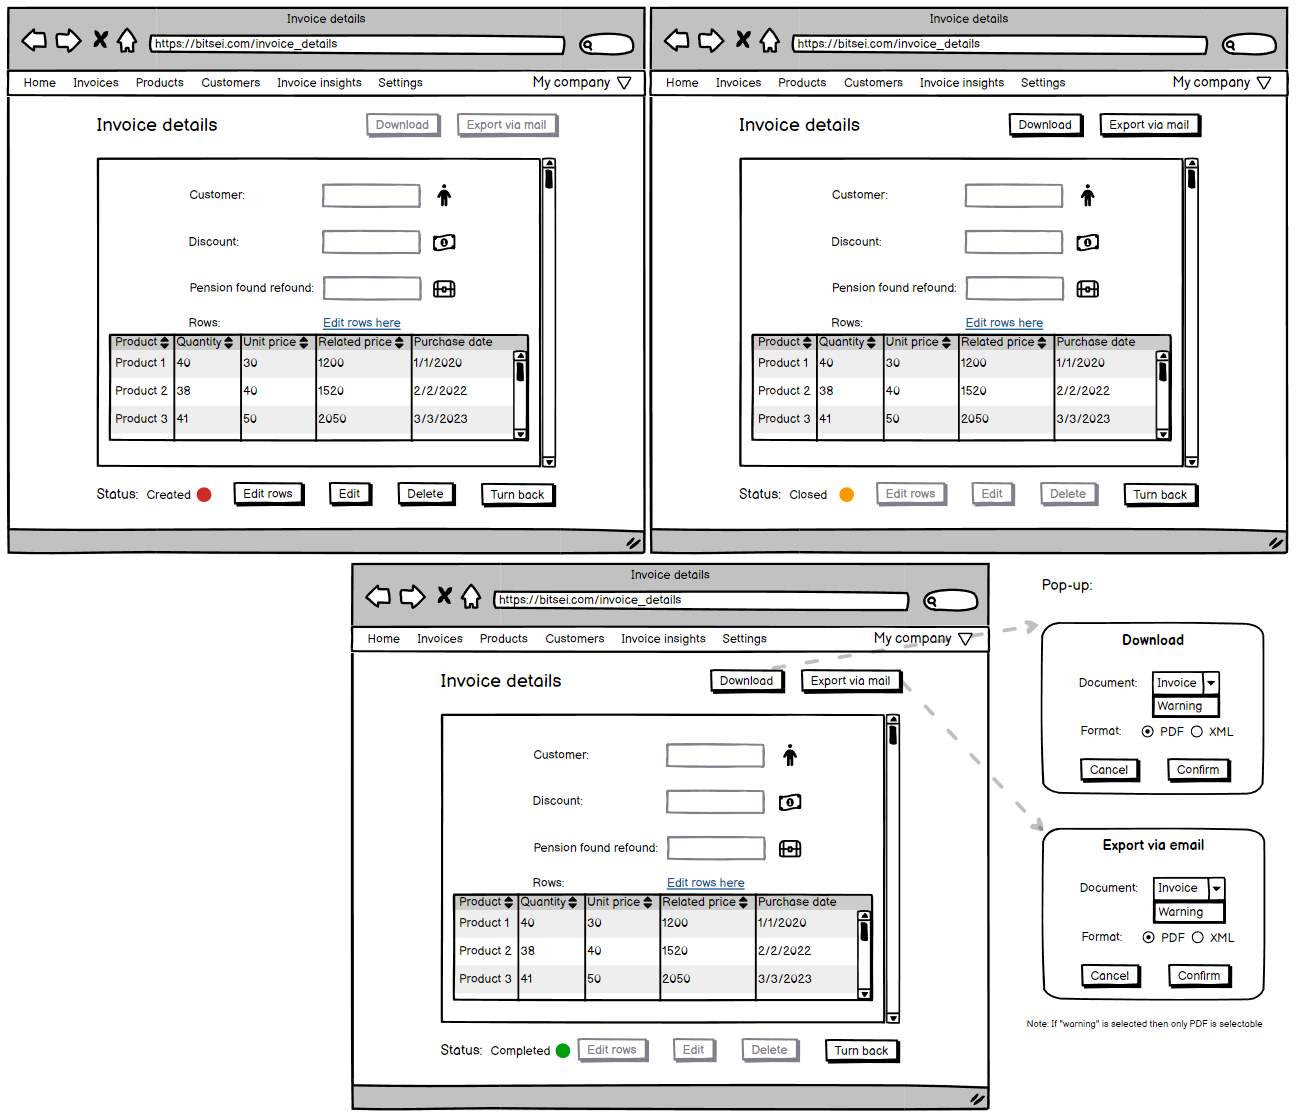
\includegraphics[height=400pt, keepaspectratio]{resources/mockup/Invoice_details.png}
\end{figure}
\newpage
\subsection{Invoice insights page}

Description

%For the main pages put a mockup and describe it in detail.
\begin{figure}[h!]
    \centering
    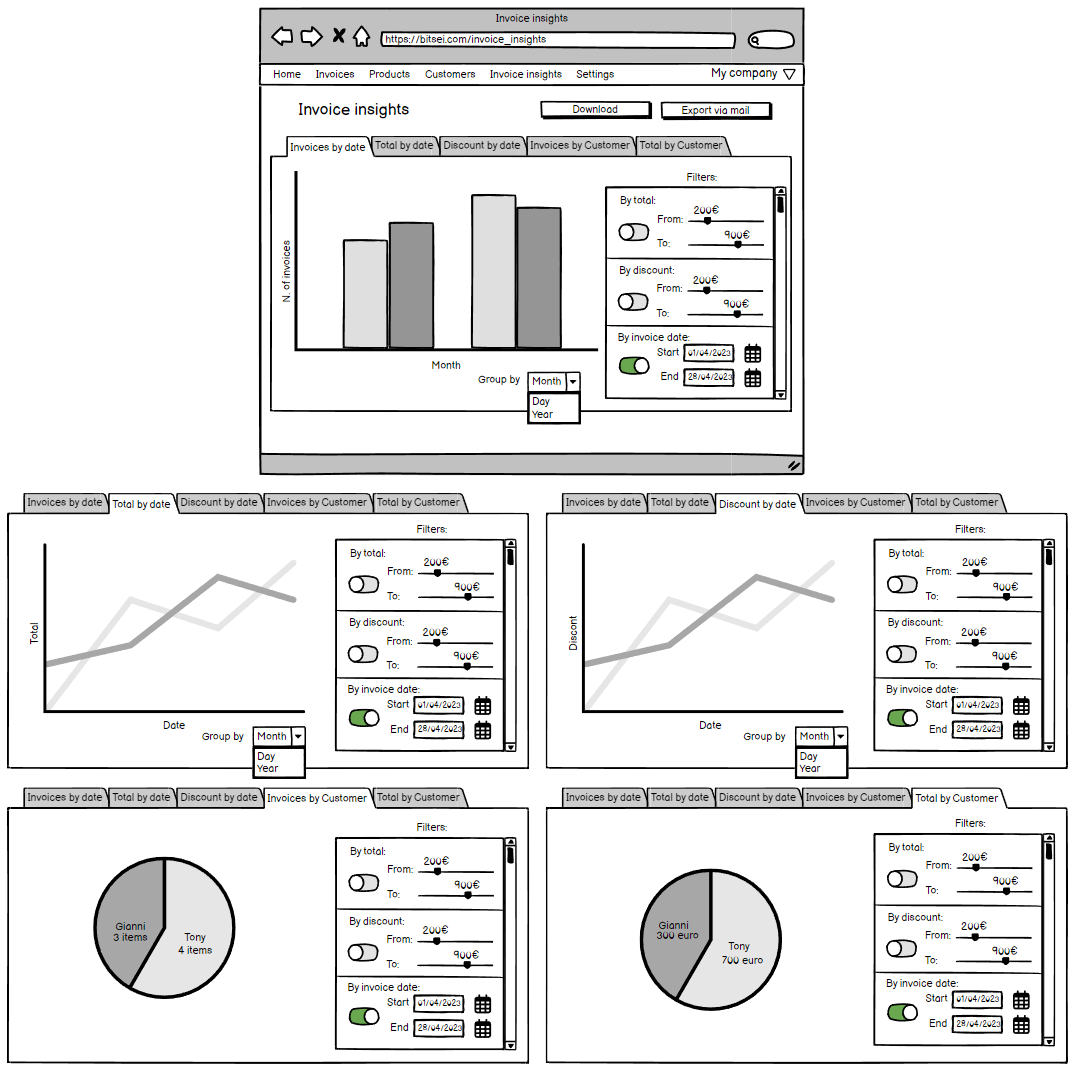
\includegraphics[height=440pt, keepaspectratio]{resources/mockup/Invoice_insights.png}
\end{figure}
\newpage
\subsection{Product list page - Create product page - Product details page - Edit product page}

Description

%For the main pages put a mockup and describe it in detail.
\begin{figure}[h!]
    \centering
    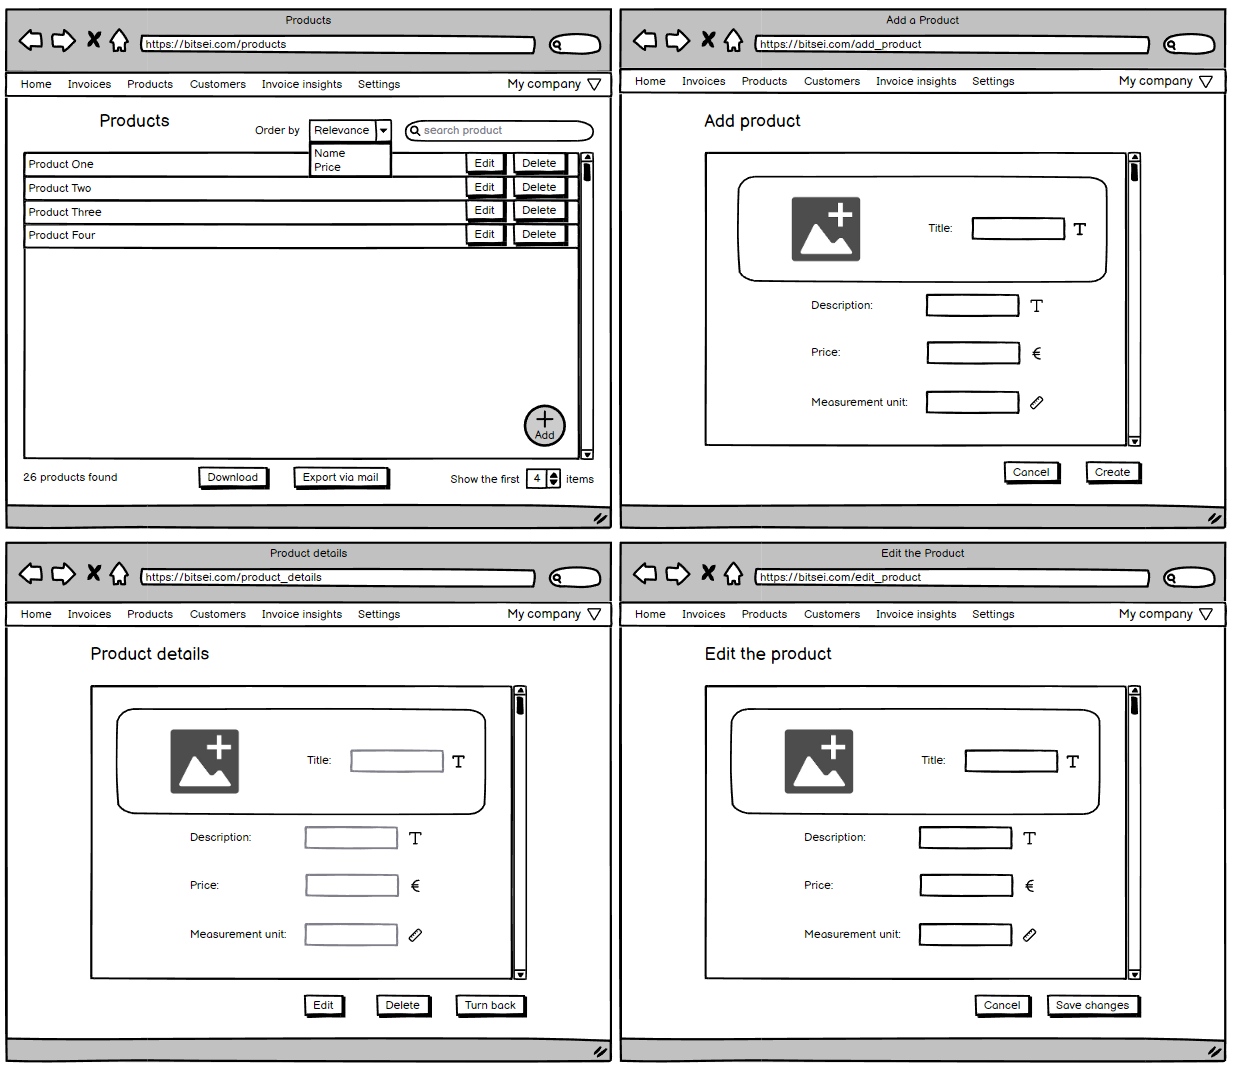
\includegraphics[height=400pt, keepaspectratio]{resources/mockup/Product.png}
\end{figure}
\newpage
\subsection{Customer list page - Create customer page - Customer details page - Edit customer page}

Description

%For the main pages put a mockup and describe it in detail.
\begin{figure}[h!]
    \centering
    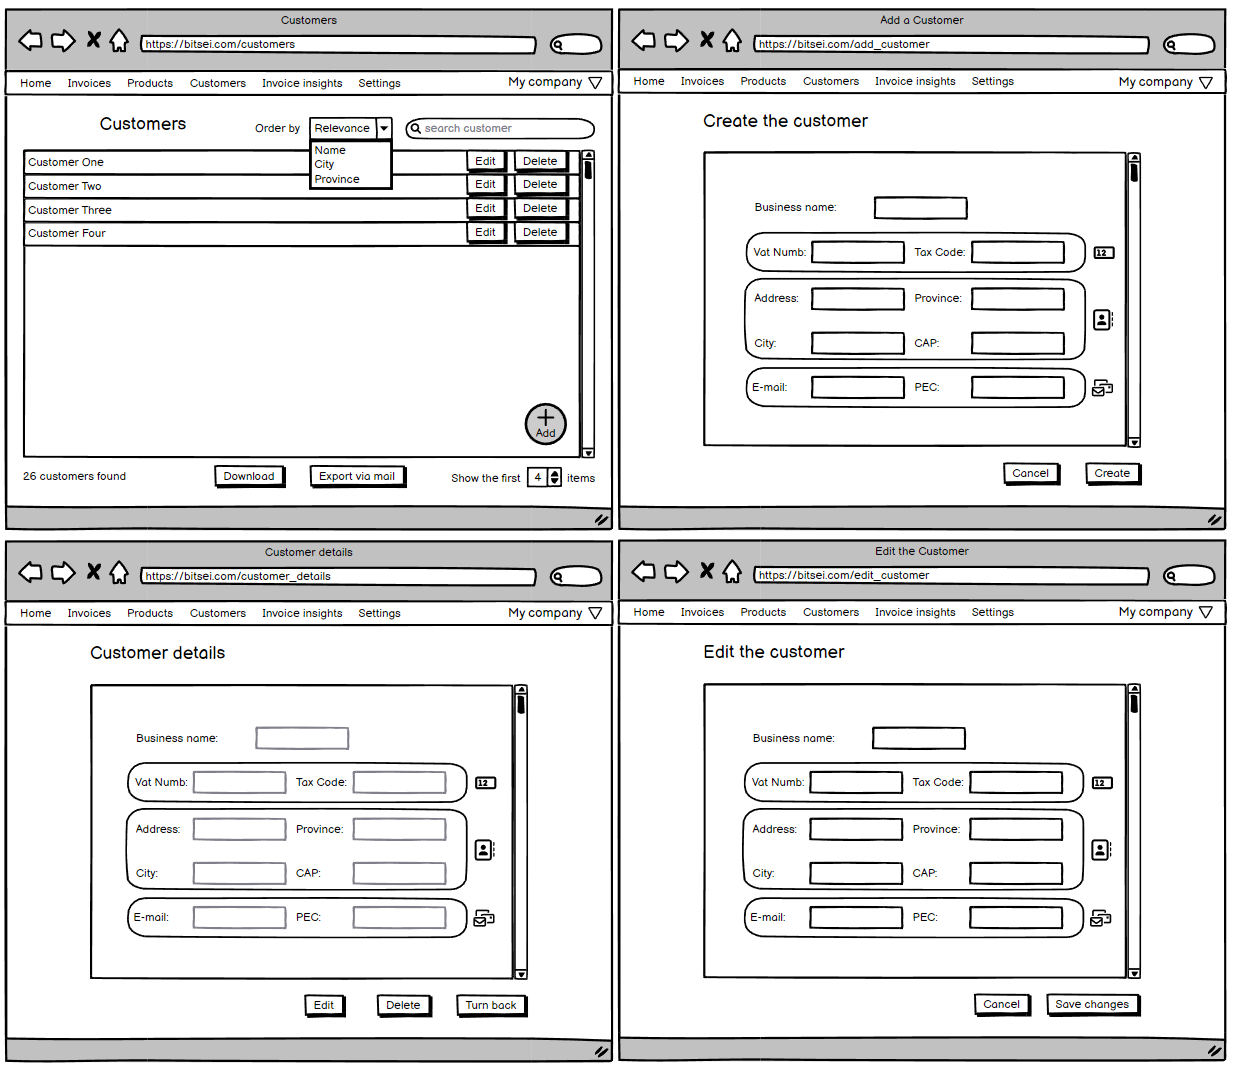
\includegraphics[height=400pt, keepaspectratio]{resources/mockup/Customer.png}
\end{figure}
\newpage
\subsection{Settings page}

Description

%For the main pages put a mockup and describe it in detail.
\begin{figure}[h!]
    \centering
    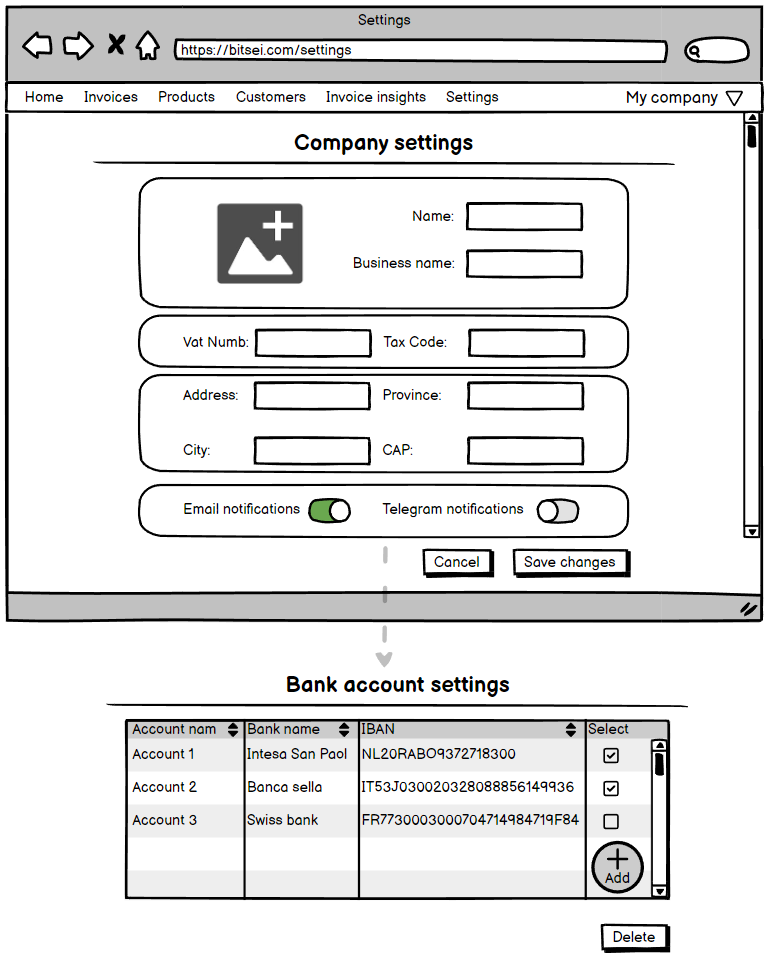
\includegraphics[height=500pt, keepaspectratio]{resources/mockup/Settings.png}
\end{figure}